%% LaTeX2e class for student theses
%% sections/content.tex
%% 
%% Karlsruhe Institute of Technology
%% Institute for Program Structures and Data Organization
%% Chair for Software Design and Quality (SDQ)
%%
%% Dr.-Ing. Erik Burger
%% burger@kit.edu
%%
%% Version 1.3.3, 2018-04-17

\chapter{Implementation}
\label{ch:implementation}

After having defined the concept for our approach as described in the previous chapter, we created a proof-of-concept prototype to evaluate our approach.
In this chapter, we describe both the visual part of the implementation and the behind-the-scenes processing which serves to prepare the data to be visualized.

The code of the implementation can be found at \url{https://github.com/gingergenius/patent-embedding-visualization}.

\section{Implementation of the data processing}
\label{sec:implementation_of_data_processing}

In this section we describe what data source we use.
We then justify our choice of programming languages and tools.
Finally, we elaborate on the data processing pipeline described briefly in \autoref{sec:pipeline}.

\subsection{Data source}
\label{subsec:data_source}

Google Patents Public Datasets \cite{IanWetherbee2017} is a data source available for public use on Google’s BigQuery platform. 
It contains full-text patent publications for the US and bibliographic data (abstract + metadata) for patents filed in the rest of the world (see \autoref{subsubsec:structure_of_a_patent_document} for the description of data fields per patent).
The database has about 100 million patent document records and is updated quarterly. 
While a quick examination of a sample of the data revealed some format errors, probably resulting from optical recognition, most of the text is readable.
This data source is therefore sufficient for a quality analysis.

We extracted four separate datasets about different technology domains from Google Patent Public Datasets:
\begin{itemize}
	\item \textit{Hair dryer} contains approximately 250 patents. It was included in the codebase from \cite{Abood2018a} and consists purely of patent applications from the US. Because of relatively small size of this dataset, separate thematic areas within it are not clearly distinguishable.
	\item \textit{Video codec} contains about 1600 patents. It was also included in the codebase from \cite{Abood2018a} and consists purely of patent applications from the US. This dataset consists overwhelmingly of patent families of different sizes. Because of that, it is suitable for evaluating how well the family similarities are handled by the semantic embeddings. However, because of our unfamiliarity with the topic of video encoding, an alternative dataset was necessary for the evaluation.
	\item \textit{3D printer} with roughly 1000 patents was produced by us using a query adapted from an existing patent landscaping report \cite{report_3d}. The full text of the query can be seen in \autoref{sec:3d_printer_query}. The dataset consists of both US and non-US patents. Non-US patents have only abstract text available while US patents have all textual fields available, of which we use the abstract and claims. We wished, however, to exclude effects resulting from different text lengths, but still make a considerable number of patents available for exploration. Consequently, we additionally prepared the contact lens dataset.
	\item \textit{Contact lens} consists of ca. 2600 patents and was based on a query adapted from an existing patent landscaping report \cite{report_lenses}. The full text of the query can be found in \autoref{sec:contact_lens_query}. We restricted this dataset to US-only patents so that we would be able to work with both the abstract and claims for the whole dataset. The contact lens dataset contains a variety of topics and is large enough for interesting exploration tasks. This is why we chose it for our evaluation.
\end{itemize}

Additionally, FIZ Karlsruhe kindly provided one more dataset extracted from the \gls{wipo} database on the topic of diesel engines (ca. 4500 patents).
The patents in it had both abstract and claims available, but no citation or family information.
Moreover, multiple languages were present in the text and everything beside English had to be filtered out.
This dataset was necessary to check how the approach performs on large data.
Unfortunately, it could not be used for the evaluation with experts because of the missing metadata attributes.

Many existing pretrained models for word embeddings are based on general vocabulary. 
Language and especially vocabulary in patent documents deviate significantly from general speech, which must be taken into account. 
Abood et. al \cite{Abood2018a} provide a word2vec model trained on 5.9 million patent documents. 
It contains a 300-dimensional embedding for each of 110239 words in its vocabulary.  
We make use of this model for our semantic analysis to compute document embeddings.

\subsection{Choice of technology}
\label{subsec:choice_of_technology}

Python \cite{python} is chosen as the programming language for preparing the data for visualization. 
It is an extremely widespread language in the field of machine learning with a great number of libraries available.
Of those libraries, Tensorflow \cite{tensorflow} in combination with Keras as a high-level \gls{api} \cite{keras} is a state-of-the-art library for neural networks. 
In fact, \cite{Abood2018a} used them in their approach for data preprocessing and for creating the word2vec model we use.
We based our approach on their codebase, so Tensorflow and Keras were also inherited by us.
Other widely used Python libraries we take advantage of are Numpy \cite{numpy} and SciPy \cite{scipy} for scientific computing and scikit-learn for machine learning.
Finally, JupyterLab \cite{jupyterlab} with an IPython \cite{ipython} kernel is selected as the development environment of choice because of ease of quick prototyping.

For the interactive visualization itself, information visualization frameworks such as Axiis \cite{axiis}, Bokeh  \cite{bokeh}, D3.js \cite{Bostock2019}, Altair \cite{altair}  and several others were considered. 
For the given problem, creating both custom user interaction techniques and custom visualization layouts consisting of new forms of charts is required. 
Unfortunately, most visualization frameworks do not support this.
Instead, they restrict the developer's alternatives to pre-determined chart types.
Coordinated interactions between views are either not supported or very limited.
Consequently, D3.js is chosen as the visualization framework with most flexibility.
It requires a hands-on, low-level approach to programming, where the developer has to manually define SVG shapes and bind their attributes such as position or color to the data.
However, this is exactly why D3.js provides the necessary level of control for the implementation of our prototype.

\subsection{Data preprocessing}
\label{subsec:data_preprocessing}

In \autoref{subsec:data_source}, we mentioned multiple datasets that were prepared for the visualization in the course of this work and the queries used to produce them.
In this section, we describe the preprocessing steps that are executed for each patent document within a retrieved dataset.

The diesel engine dataset was, unlike the others, not derived from Google Patents Public Datasets, so it required some minor additions to the pipeline.
The data structure was slightly different and therefore had to be transformed for compatibility.
Moreover, the patent texts had to be cleaned as there were some \gls{xml} tags present that we removed.
Additionally, the diesel engine dataset included a non-negligible amount of text in French and German within the patent claims. 
To filter out non-English text, we split the text into sentences and detected their language using the Python library langid \cite{Lui2012}.
This language detection tool utilizes a multinomial naive Bayes classifier trained on n-grams to reliably produce a robust result independently of domain and text length \cite{Lui2011}.

The interviews with the patent experts indicated that title, abstract and claims are the most valuable textual parts of a patent document for understanding the described invention.
Other textual parts, such as background art or description of figures, do not contribute significantly to the essence of the invention.
Therefore, for all further steps we concatenate the patent's title, abstract and, when available, its claims.
This way, we maximize the length of relevant textual content taken into account.
We do not consider the three above-mentioned textual fields separately for sake of simplicity.
However, for future work it might be worth examining how different textual parts of the same document compare to each other when semantic methods are applied to them separately.

\paragraph{Tokenization}~\\
The proper preprocessing starts with \textit{tokenization}, which means splitting the text into tokens.
Tokens in our case are not characters or sentences but words since we use word embeddings from a pre-trained word2vec model.
We use a \verb|Tokenizer| class from Keras which replaces all punctuation except the apostrophe character with spaces.
It then translates the whole text to lowercase and splits the text into words divided by spaces.
The last step is replacing the numbers that occur separately or as parts of a word with a \verb|_NUMBER_| token. 

\paragraph{Stopword removal}~\\
After we have successfully tokenized the data, the next step in the pipeline is the stopword removal to increase the amount of meaningful information per document.
We use two stopword lists: one is a general list of English stopwords from Natural Language Toolkit \cite{bird2009natural} and the other one is a patent-specific list kindly provided by FIZ Karlsruhe.
The latter list includes words like ``comprised'', ``abovedescribed' and ``obtained'' which often appear in patent texts and do not contribute to the meaning.
Words shorter than 3 characters or longer than 50 characters are eliminated as well.
Finally, when the number of meaningful words per patent becomes clear, we remove all patent documents that contain less than 30 words.
The amount of the remaining text at this stage varies between the datasets, but in all cases it followed a left-skewed distribution with a mode of approximately 250 words and an average of 500 up to 1000 words.
Distributions for diesel engine and contact lens can be found in \autoref{fig:text_length_distributions}.
 
\paragraph{Parsing of metadata attributes}~\\
This step is independent of the processing of textual content, but instead prepares the metadata attributes for visualization.
Metadata attributes such as references, assignees and \gls{ipc} classes are included in the data as a string made up of comma-separated values, so we split the list to get each separate value.
For \gls{ipc} classes, we compute a list of unique codes for all levels of the \gls{ipc} hierarchy per document (see \autoref{table:ipc_classes_structure} for description of levels).

The assignee names present a challenge with regard to the data quality.
Institutions' legal names are written out in a very inconsistent way throughout the data.
There are often multiple variants with parts of the name which are abbreviated in some cases but not in others.
Different branches or subsidiaries of the same company are also often present.
Lastly, there are errors and misspellings as well, partly as a result of \gls{ocr} artifacts.
This last point applies to assignee names signifying private persons as well as companies.

We would like to be able to reliably group patents by their assignees.
For this, we merge similar assignee names with \textit{fuzzy string matching}, which is a technique of finding strings that are approximately the same.
We use the Python library \verb|FuzzyWuzzy| \cite{Cohen2011}, which is based on Levenshtein distance between two sequences of characters.
The Levenshtein distance is a measure of similarity composed of the number of character deletions, insertions or substitutions required to transform one string into another \cite{levenshtein}.
The value returned by the library is not the absolute distance but a similarity percentage that takes string length into account.
We use a simple similarity threshold of 88\% to determine which assignees to combine into one entry.
The threshold value was chosen empirically to provide sufficiently good results.
Fuzzy string matching allows us to reduce the number of unique assignees in the dataset by 10-15\%.
However, false positives (match detected where none exists) and false negatives (existing match not detected) could not be completely excluded from among the matches.

\subsection{Sunburst hierarchies}
\label{subsec:hierarchies}

As we would like to use the sunburst control for arbitrary combinations of metadata attributes, corresponding hierarchical aggregations need to be computed.
For that, we consider \gls{ipc} class, country, assignee by themselves and also all possible permutations (orderings) of those attributes of size two.
We do not consider stacking all three attributes as sunburst levels because of space restrictions and because the groups after the third division would become very small.
However, it would only be effective for larger datasets and documents with multiple non-hierarchical metadata attributes.

For metadata attributes, we distinguish between a single value per document (e. g. country), a list of values per document (e. g. assignee) and a hierarchical code such as an \gls{ipc} code or a list of such codes.
This allows us to adjust how the aggregation is computed depending on the type of the attribute.
For \textit{value attributes}, we can just group all documents by their unique values of the corresponding attribute.
For \textit{list attributes}, a single document can be referenced in multiple hierarchy nodes, so it should be counted multiple times.
\textit{Code attributes} are essentially multiple list attributes in a certain order (section, class, subclass, group, subgroup) with one extra condition: a subclass from one \gls{ipc} code (for example, N04N) can only count as a child of its own class (N04) and not some other class (B02).

As mentioned in \autoref{subsubsec:sunburst}, because patents simultaneously belong to multiple nodes, a total number of patents in the hierarchy may exceed the size of the dataset.
In this case, the values of all nodes are normalized so that they yield 100\% when combined.
The normalization starts from the shallowest hierarchy level and then goes into the depth.

\subsection{Key term extraction}
\label{subsec:term_extraction}

We extract relevant key terms per document so that the user can get a first impression of the content of a document with just a quick glance.
For this extraction we use \gls{tf-idf} which is a widely used weighting technique to determine most important words or phrases in a corpus.
Essentially, the more often a phrase occurs in a document, the most important it is for this document (\gls{tf}).
At the same time, the more often the same phrase occurs throughout the whole document corpus, the less explanatory power it has (\gls{idf}).

For our data, unigrams (single words) and bigrams (two-word phrases) produce most meaningful results.
To exclude extremely rare terms and spelling mistakes, only phrases that occur in more than ten documents are considered for their relevancy.
Additionally, we also explicitly exclude terms appearing in over 20\% of the corpus from consideration because they are unlikely to result in an information gain.
For each patent, we save a list of ten terms that were most highly ranked by \gls{tf-idf} for visualization.

\subsection{Embeddings}
\label{subsec:embeddings}

\paragraph{Document vectors}~\\
The purpose of this stage is to produce a representation of a document based on the words it consists of.
The input of this step is a sanitized list of words per patent, which is a result of the tokenization and stopword filtering operations described in \autoref{subsec:data_preprocessing}.
We compute each document embedding as a weighed average of the embeddings of words the document contains.
300-dimensional word embeddings are retrieved from the pre-trained word2vec model provided by \cite{Abood2018a}.
The weighting factor for each word is its \gls{idf}, which at this point had already been computed as described in \autoref{subsec:term_extraction}.
Adjusting the weight of a word by its frequency in the corpus takes the varying importance of separate words into consideration and therefore helps capture themes in the dataset in a better way.
Weighting with \gls{idf} has been successfully used for computing semantic similarity \cite{Zhao2015} \cite{NAGOUDI2018}, \cite{Arora2017} and for sentiment analysis \cite{Correa2017}.
In our case, we found that compared to non-weighted word averages, weighted word vectors result in a clearer separation of clusters after dimension reduction compared to non-weighted word vectors.
The documents were more likely to gather into dense groups instead of being distributed uniformly.
A comparison of weighted and non-weighted word averages can be seen in \autoref{fig:weighted_vs_average_diesel} and \autoref{fig:weighted_vs_average_contact_lens}.

\begin{figure}[!]
    \centering
    \subfigure[Non-weighted average]
    {
        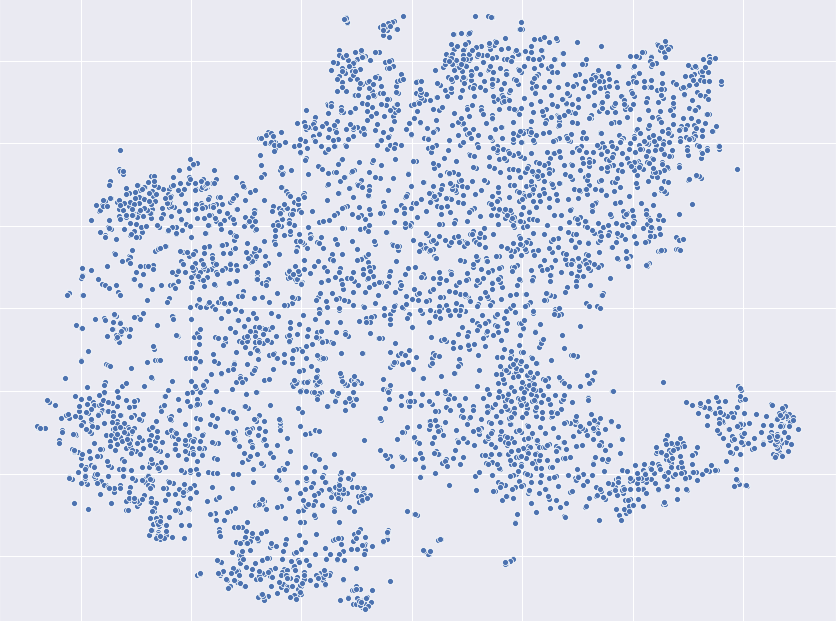
\includegraphics[width=0.95\textwidth]{img/diesel_avg}
    }\\
    \subfigure[Weighted average]
    {
        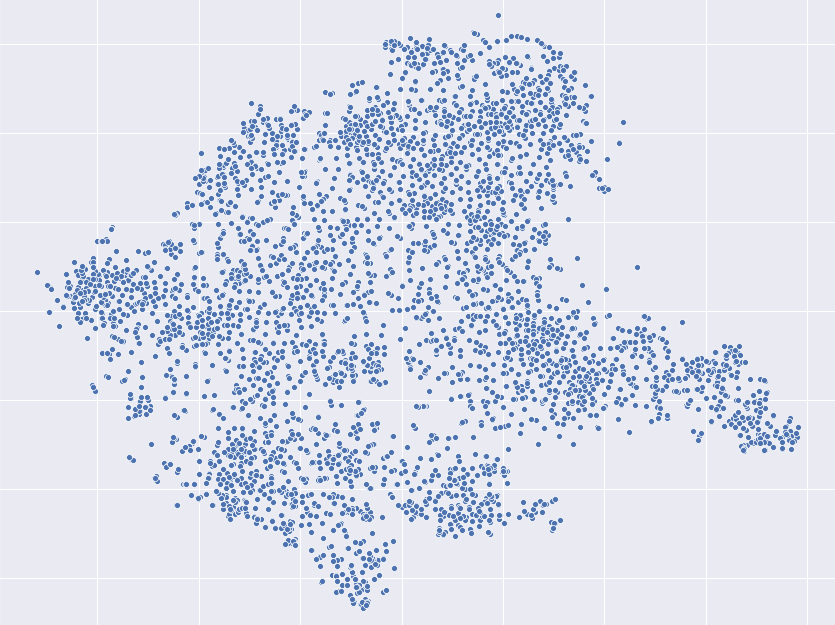
\includegraphics[width=0.95\textwidth]{img/diesel_weighted}
    }
    \caption{A comparison of document vectors computed with and without \gls{idf} weighting. Diesel engine dataset.}
    \label{fig:weighted_vs_average_diesel}
\end{figure}

\paragraph{Dimension reduction}~\\
Points in a very high-dimensional space are not suitable for an understandable visualization.
For the purposes of visualization we need to transform document vectors into a two-dimensional space so that any patterns in the data become recognizable.

We compared multiple dimension reduction techniques such as metric and non-metric \gls{mds} \cite{OConnell2006}, Isomap \cite{Tenenbaum2000}, \gls{pca} \cite{hotelling1933analysis}, \gls{umap} \cite{McInnes2018} and \gls{tsne} (see \autoref{subsubsec:tsne}).
In the interviews, patent experts emphasized that patents from the same family possess a great degree of semantic similarity and one should expect them to be placed closely to each other (see \autoref{subsec:implications}).
Handling patent families correctly is a minimum requirement for a suitable dimension reduction technique.
For this reason, the comparison was conducted on the video codec dataset since it chiefly consists of patent families of different sizes.

Among the tested dimension reduction techniques, \gls{tsne} was the only one in which families were clearly identifiable and separated from their surroundings.
Figure \autoref{fig:tsne_video_codec} shows numerous ``clumps'' of closely situated points.
Further inspection showed that they mostly belonged to the same family, even when the family information present in the dataset was incomplete and did not explicitly list a connection.
In the majority of other cases, the patents within the groups belonged to the same assignee, dealt with the same invention and were therefore textually very similar (see Figure \autoref{fig:tsne_video_codec_double}).
When tested with other datasets, \gls{tsne} resulted in easily identifiable accumulations of points distinctly separated from each other by empty areas.
Other techniques were apt to clump the points into one big area or distribute them uniformly without defined groups.
Large sparse zones consisting purely of apparent outliers were also likely to appear.
For comparison, see \autoref{fig:other_dimension_reduction} for the results from other dimension reduction methods.

\begin{figure}[!]
    \centering
    \subfigure[The result of the dimension reduction by \gls{tsne}. The points are plotted in the same color and size to make close groups visible]
    {
        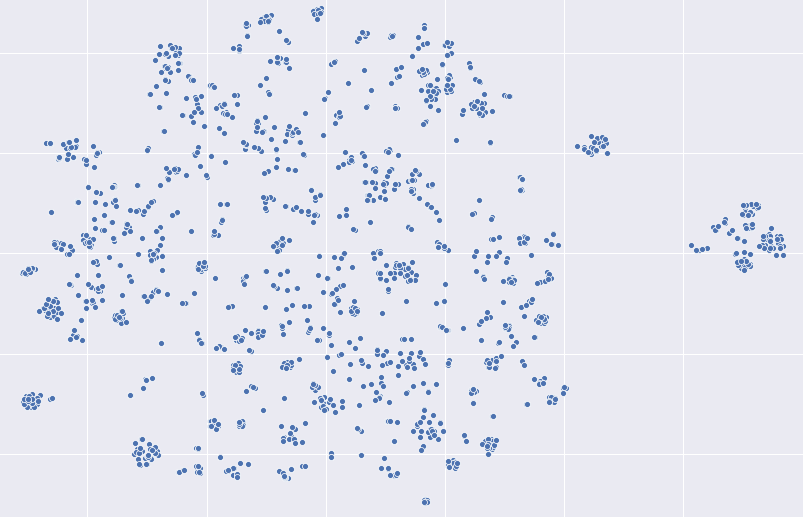
\includegraphics[width=\textwidth]{img/tsne_video_codec}
        \label{fig:tsne_video_codec}
    }\\
    \subfigure[Same coordinates as above, displayed in the interactive prototype. The patents from the same assignee are drawn in the same color, which shows that groups constitute patent families]
    {
        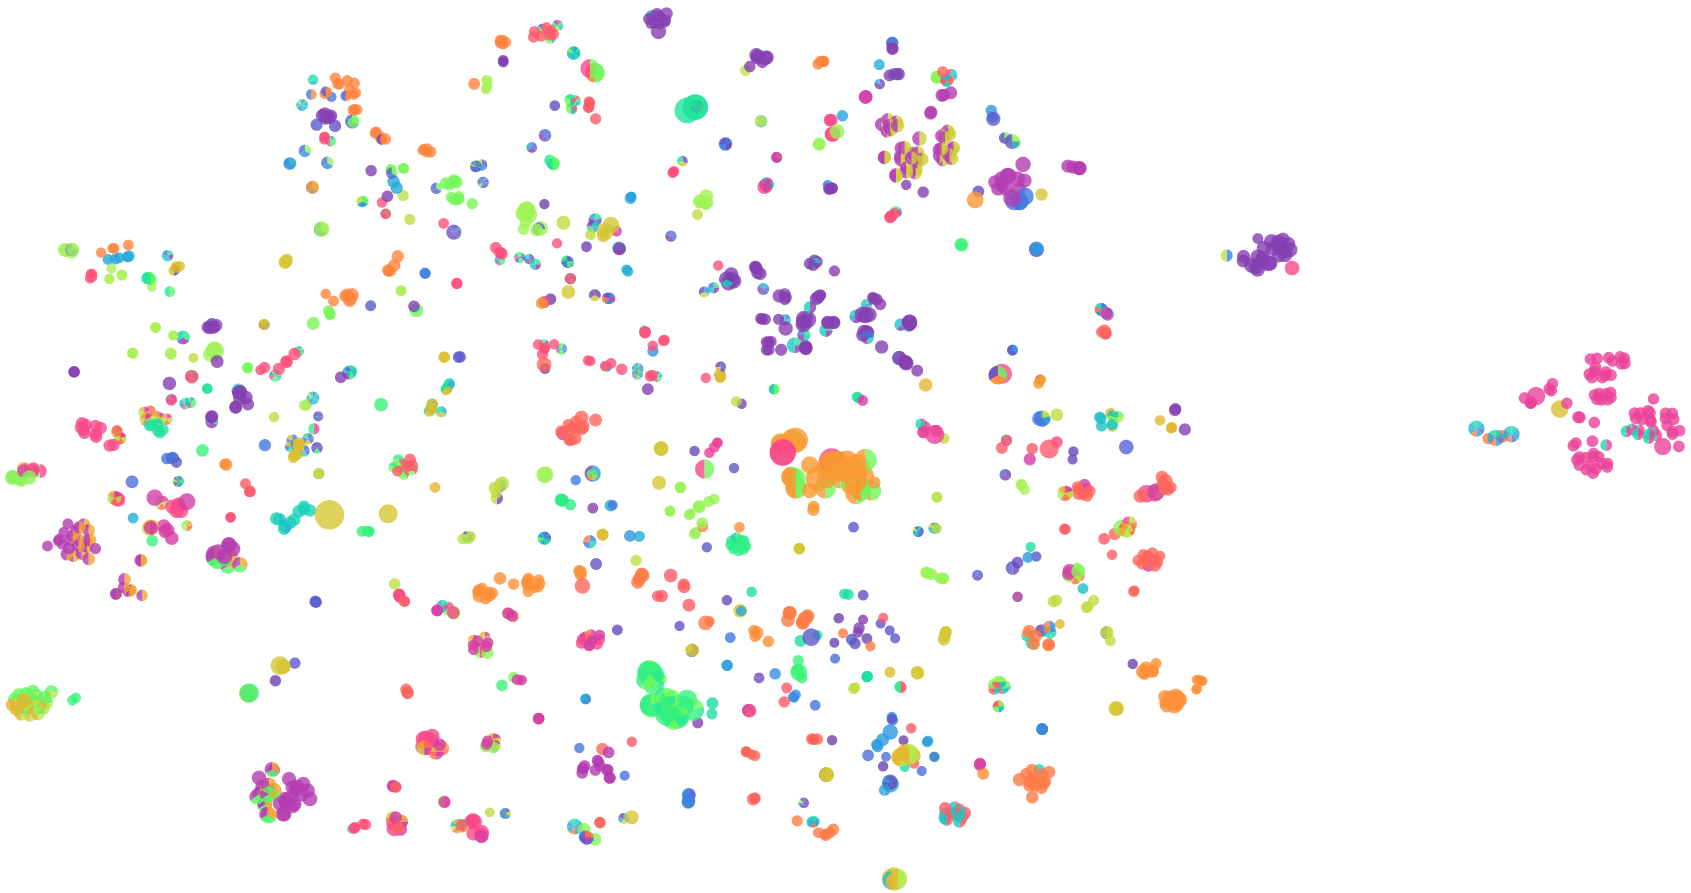
\includegraphics[width=\textwidth]{img/tsne_video_codec_assignees}
        \label{fig:tsne_video_codec_assignees}
    }
    \caption{The result of dimension reduction by t-SNE on the video codec dataset.}
    \label{fig:tsne_video_codec_double}
\end{figure}

As \gls{tsne} tries to retain distances from the high-dimensional space in the lower-dimensional representation (see \autoref{subsubsec:tsne} for details), a suitable \textit{distance metric} has to be used.
Distances in high-dimensional spaces behave in a non-intuitive way and currently there is no consensus on the ``best'' metric for all possible applications.
We experimented with multiple distance metrics such as euclidean distance, cosine similarity and manhattan distance.
The local structure of the data seemed stable independently of the used metric, only the relative placement of larger groups changed.
Ultimately, we settled on \textit{cosine similarity}, which is widely used in \gls{nlp} applications.
For two vectors A and B, cosine similarity is measured as the cosine of the angle between them.
It can be derived easily using a dot product as shown in \autoref{eq:cosine}.

\begin{equation} \label{eq:cosine}
\mathbf{A} \cdot \mathbf{B}=\|\mathbf{A}\|\|\mathbf{B}\| \cos \theta
\end{equation}

As a result of this stage, 300-dimensional document vectors have been transformed into two dimensions for visualization using \gls{tsne} with cosine similarity as a distance metric.

\subsection{Hierarchical clustering}
\label{subsec:hierarchical_clustering}

At this step we have 2D coordinates of all patents, but it is not immediately clear to the user why they are placed in a certain way. 
To explain the semantic similarities within groups at multiple levels of detail, we use agglomerative (bottom-up) \textit{hierarchical clustering}.
Essentially, is a process in which every data point is considered its own cluster at the beginning. 
Those singular clusters are then merged into their nearest clusters  one-by-one, and in the following iterations, clusters join the adjacent clusters until the whole dataset is joined into one single cluster.
The changes are tracked throughout the algorithm within a \textit{distance matrix}, in which pairwise distances between any two clusters are stored.
The process constructs a tree called \textit{dendrogram} which reflects the structure present in the distance matrix.

An example dendrogram is shown in \autoref{fig:example_dendrogram}.
Points E and F are the nearest pair of points in the dataset, so they are combined to a cluster EF on the first iteration of the algorithm.
The same thing happens to A and B on the second iteration.
Point D and subsequently point C join cluster EF and finally, cluster AB and cluster CDEF are merged to create a root node of the hierarchy.
Since it is a tree structure, there is no single correct number of clusters in a hierarchical clustering.
After every merge one can decide to make a ``cut'' as shown by the orange line.
At this specific level of detail, the dataset is then divided into a number of clusters equal to the number of dendrogram lines the cut crosses.

\begin{figure}[!]
\centering
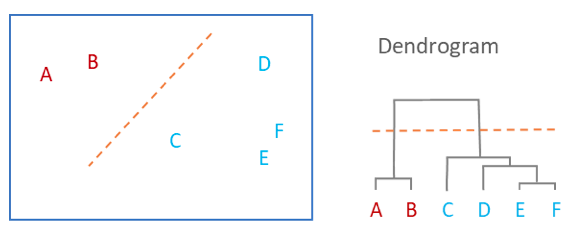
\includegraphics[width=0.7\textwidth]{img/example_dendrogram}
\caption{An example of dendrogram used in hierarchical clustering and its input data. Image source: \cite{Bock}}
\label{fig:example_dendrogram}
\end{figure}

A distance between any two points is clearly defined in a 2D space, but multiple definitions exist for distance between two clusters.
SciPy's \verb|linkage| method, which we used as an implementation of the hierarchical clustering, offers various options for calculating the distance between two clusters:
\begin{itemize}
	\item \verb|single| (Nearest Point Algorithm) uses the minimal distance between points from different clusters
	\item \verb|complete| (Farthest Point Algorithm) uses the maximal distance between points from different clusters
	\item \verb|average| uses $d(u, v)=\sum_{i j} \frac{d(u[i], v[j])}{(|u| *|v|)}$ where $u$ and $v$ are the two clusters and |u| and |v| are their respective cardinalities
	\item \verb|weighted| uses $d(u, v)=(d i s t(s, v)+d i s t(t, v)) / 2$ where clusters $s$ and $t$ were previously combined to form $u$ and $v$ is the remaining cluster
\end{itemize}

To identify the best algorithm, we computed a Cophenetic Correlation Coefficient \cite{sokal} for all above-mentioned algorithms on all five of our datasets.
The coefficient compares (correlates) the actual pairwise distances of all data points to those implied by the hierarchical clustering. 
The closer the value is to 1, the better the clustering preserves the original distances. 
The method \verb|average| consistently produced higher values of Cophenetic Correlation Coefficient across the datasets, which made it our preferred method.

Besides clustering in 2D space after the dimension reduction, we experimented with clustering in the original 300-dimensional document space as well.
The resulting structures were not preserved well during the dimension reduction.
The clusters were not clearly divided, which means it was impossible to draw a clear boundary between clusters.
This led to problems with placing cluster labels as described in \autoref{subsubsec:clusters}.
We therefore prefer clustering data in the same space where it is visualized.
This is due to a compromise that has to be made between representing the structures in the original high-dimensional space accurately and keeping the end result sufficiently simple for human cognition and therefore interpretable.

An example of a resulting dendrogram is shown in \autoref{fig:dendrogram_contact_lens}.
We manually chose three levels of detail for each dataset according to consistent principles.
We refer to the levels of detail in terms of \textit{large}, \textit{medium} and \textit{small} clusters.
\begin{itemize}
\item The number of large clusters should be between 3 and 7 depending on the structure of the dataset. 
At this level the most general topics in the dataset should be visible.
\item The number of medium clusters should be between 10 and 20, so that every large cluster is divided into approximately 3 to 4 smaller topics.
\item The number of small clusters should be between 40 and 70, so that every medium cluster is divided into 3 to 4 parts.
This finest level of detail is aimed at summing up patent families and very closely related inventions.
\end{itemize}
An example separation of a dataset into large clusters is presented in \autoref{fig:contact_lens_large}.

\begin{figure}[!]
\centering
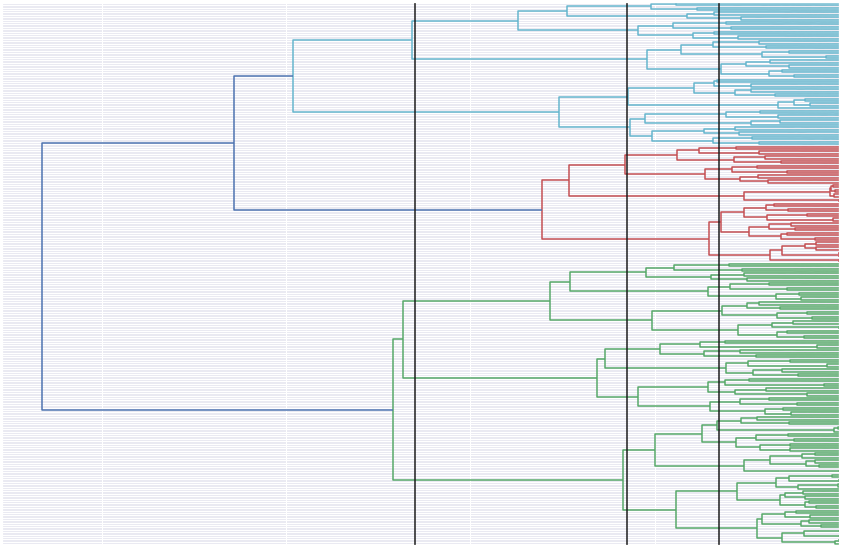
\includegraphics[width=\textwidth]{img/dendrogram_contact_lens}
\caption{Dendrogram computed on the contact lens dataset. The cutoff values for three detail levels are shown in black.}
\label{fig:dendrogram_contact_lens}
\end{figure}

\begin{figure}[!]
\centering
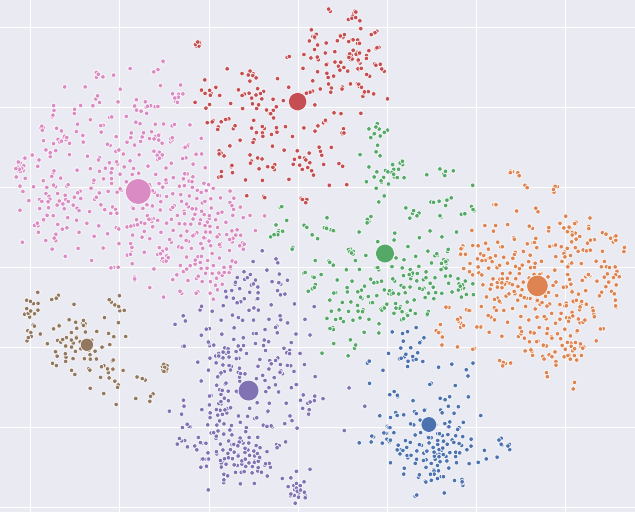
\includegraphics[width=\textwidth]{img/contact_lens_large}
\caption{The most abstract detail level (large clusters) of a clustering on the contact lens dataset. Each cluster has its own color. The circles represent cluster centroids and their radius corresponds to the number of documents within the cluster.}
\label{fig:contact_lens_large}
\end{figure}

To make the similarities between patents within a cluster explicit for the user, we summarize key terms from documents within the cluster to a list of cluster key terms.
As described in \autoref{subsubsec:points} ``Labels'', patent documents are characterized by a list of the 10 most relevant key terms as computed by \gls{tf-idf}.
Across the cluster, we count the occurrences of each term within those 10 document terms.
The 15 most frequently occurring key terms are considered most relevant for the given cluster.
This approach results in more general and common key terms for large clusters, with the specificity growing with each level of detail.

As described in \autoref{subsubsec:clusters}, we augment cluster key terms with similar words to put them into context and avoid ambiguity.
For that, we extract the 10 most similar words from the word2vec model used previously as candidates.
Most similar in this case means that the cosine similarities between word embedding vectors are maximal.
This is the most computationally expensive step in the pipeline since the similarity has to be computed for every single word in the model's vocabulary and for every cluster key term.
If a candidate appears in more than 10\% of documents in a cluster, it is considered an adequate enhancement for the given cluster key term.
Since the word2vec model we use only takes single words into account and does not contain embeddings for multi-word units, bigrams cannot be augmented this way.

The interviews with the patent experts showed that during a patent search, they describe the concept they search for in different levels of abstractness, e. g. umbrella terms and narrower terms (see \autoref{subsec:participant_alpha} and \autoref{subsec:participant_gamma}).
To aid the user's understanding of key terms we attempted to produce generalizations of cluster key terms which are called \textit{hypernyms}.
For example, \textit{chair} is a kind of \textit{furniture}, so \textit{furniture} is a hypernym for \textit{chair}.
These kinds of relationships between words in the English language have been manually captured in the WordNet database \cite{wordnet}.
Our attempt resulted in very similar hypernyms for all clusters that were too general to be useful, for example \textit{speed, base, length, element, metal, gas, velocity, constant, concentration}.
For this reason, we did not pursue this research direction further.

\section{Implementation of the user interface}
\label{sec:user_interface_concept}

In this section, we describe each component of the proposed visualization layout separately.
We examine how the dimensions of data are mapped to visual attributes.
We then describe how the views are coordinated through the way they react to user interactions.

A schematic representation of the visualization layout is shown in \autoref{fig:schematic}.
The layout consists of two columns and each of them is split into two rows as shown in \autoref{fig:columns_rows_layout}.
The first column takes 75\% of the screen's width and contains the scatter plot (80\% of the total height) and the histogram (20\% of the total height).
The second column fills the remaining 25\% of the total width and contains the sunburst with breadcrumbs in the top two-thirds and the detail view in the bottom third.
In the early versions of the prototype, the width and height of the layout's elements were fixed.
Later, we switched to relative sizes to become independent of the exact screen dimensions.
Nevertheless, the prototype is best viewed within a range of resolutions from 1600x900 to 1920x1080 pixels on a screen diagonal from 14 to 24 inches.
The main restriction to arbitrary scalability are the font sizes used in the user interface.
With resolutions smaller than mentioned above the overlap between text elements is likely to harm readability.
With larger resolutions text and point elements will be too small, but it can be alleviated by magnifying the whole web page.

\begin{figure}[!]
\centering
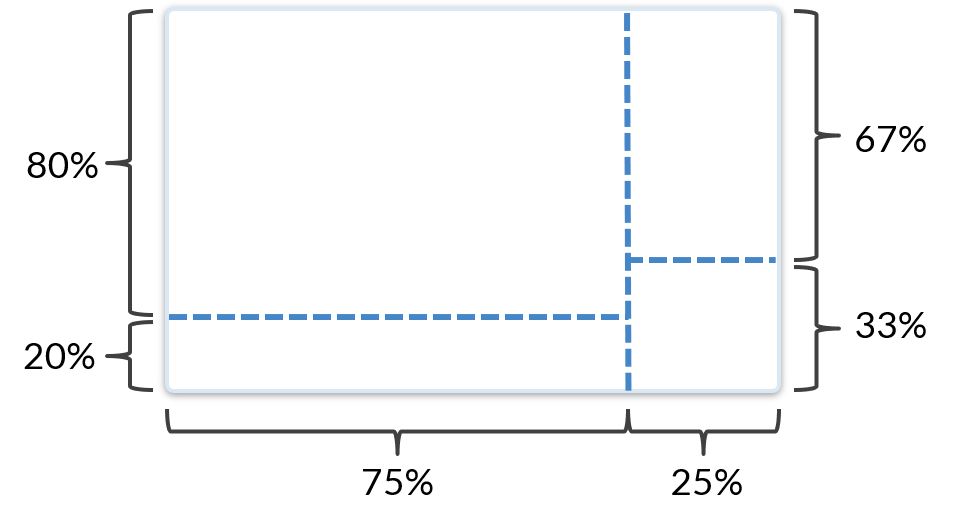
\includegraphics[width=0.6\textwidth]{img/columns_rows_layout}
\caption{Proportions of rows and columns in the dynamic layout.}
\label{fig:columns_rows_layout}
\end{figure}

\subsection{Scatter plot}
\label{subsec:scatter_plot}

The scatter plot is the main area of the visualization and is complemented by all other elements: histogram, sunburst + breadcrumbs and detail view.
It represents each patent as a point with coordinates that correspond to its position after dimension reduction with \gls{tsne}.
Additionally, points are grouped into clusters, each of which is indicated by its key terms.
In this subsection we discuss the depiction of single patents first. 
We then proceed to describe cluster representations.

\subsubsection{Points}
\label{subsubsec:points}
Each data point possesses multiple visual dimensions: position, size, color. 
In the following paragraphs we describe how they are mapped to dimensions of the data.
As mentioned before, the position corresponds to the coordinates in the semantic document space reduced to two dimensions.
Size and color are also utilized (see ``Size'', ``Color and glyphs'').\todo{cite suitability of visual dimensions}
They are complemented by connections between patents (see ``Connections'').
Lastly, each point is labeled with the top key terms of the corresponding patent.

\paragraph{Size}~\\
The size of a point depends on the number of forward and backward citations the patent has, all summed up.
The radius of the circle varies between 3 and 9 pixels when no zoom is applied.
The exact scale used in this mapping is dynamic and dependent on the dataset. 
The minimum size always corresponds to the lowest number of citations found per patent in the dataset and the maximum size to the highest number.
The interpolation between the two values is linear.
It is not uncommon for a patent to list hundreds of citations.
With this relative scale, we make sure that the size difference is always obvious to the user, regardless of whether the maximum number of citations per patent in the current dataset is 20 or 900.

\paragraph{Color and glyphs}~\\
Color of the points is a dynamic variable which is defined by the current state of the sunburst's hierarchy.
Specifically, whenever the user navigates to a different sunburst node, colors are newly assigned for its child nodes.
Patents that are outside of the scope of the current node are then completely hidden.
The remaining points in the scatter plot obtain their color depending on their value of the corresponding metadata attribute.

Earlier iterations of the prototype did not include a solution for displaying patents with multiple values of the given attribute.
Instead, they were assigned to the color of the least frequent attribute value.
The intuition behind this solution was to provide visibility to a group that otherwise would be less noticeable, especially if those least frequent values only occur in combination with others.

Eventually, we implemented \textit{glyphs} as a solution for the issue of multiple attribute values.
``A glyph is a graphical object designed to convey multiple data values'' \cite{ware2004information}.
Usually, glyphs possess multiple visual attributes such as color, position or length, which are mapped to different dimensions of the data.
In our case, however, they are restricted to depict only one dimension of the data, which can acquire one or more values.

Our proposed glyphs are depicted in the form of pie charts with a number of slices corresponding to the number of attribute values.
The slices are equally sized since all values of a given attribute are equally meaningful.
Since we wanted to keep the patent representations uniformly shaped, a circular multi-colored pie chart was an obvious enhancement of a single-colored circle.
The idea was also partially inspired by \cite{Dou2011}, where pie glyphs show the distribution of topics within a document. 

Naturally, the question about legibility of pie charts arose. 
If they were to contain too many slices, they would be impossible to decipher.
To check this, we computed the distribution of how many different values patents included for assignees and \gls{ipc} classes (see \autoref{fig:list_distribution}).
The values presented were computed on the contact lens dataset which is described in \autoref{subsec:data_source}, but they do not vary greatly between datasets.

On average, there are 1.56 assignees per patent, with an overwhelming majority of patents having only one assignee.
\gls{ipc} classes on the first glance look unsuitable for a pie chart with an average of 4.92 \gls{ipc} classes per document and a non-negligible amount of patents with more than 20 \gls{ipc} classes.
However, these numbers refer to unique \gls{ipc} classes throughout the whole \gls{ipc} hierarchy.
In reality, only one \gls{ipc} level is visible at one time, so we examined distributions after the first subdivision and before the last one to see how many classes truly have to be shown simultaneously.
On the subdivision level with single \gls{ipc} letters (e.g. A or B) there is an average of 1.87 values per patent, and on the group level (e.g. A21B1 vs. A21C3) it is 3.34, respectively.
This shows that in total, there is relatively little branching throughout the \gls{ipc} hierarchy with most of it happening on the last level. 
This means that the number of slices in a pie chart on each specific \gls{ipc} level is not too high for intelligibility.

\begin{figure}
    \centering
    \subfigure[Assignee]
    {
        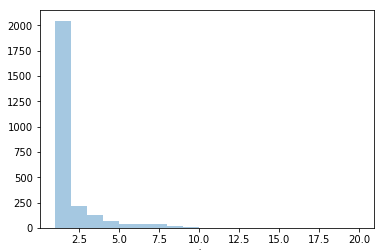
\includegraphics[width=0.45\textwidth]{img/assignees_distribution}
        \label{fig:assignees_distribution}
    }
    \subfigure[\gls{ipc} class]
    {
        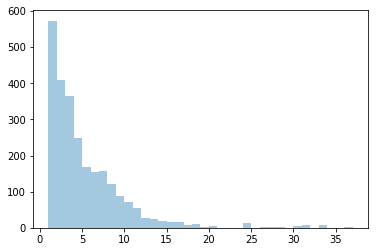
\includegraphics[width=0.45\textwidth]{img/ipc_classes_distribution}
        \label{fig:ipc_classes_distribution}
    }\\
    \subfigure[First letter of \gls{ipc} class (section)]
    {
        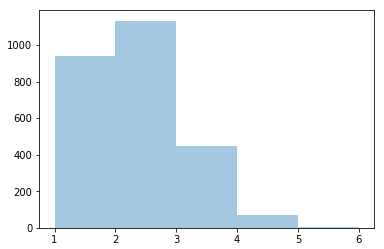
\includegraphics[width=0.45\textwidth]{img/first_letters_distribution}
        \label{fig:first_letters_distribution}
    }
    \subfigure[\gls{ipc} class on group level (4-6 characters)]
    {
        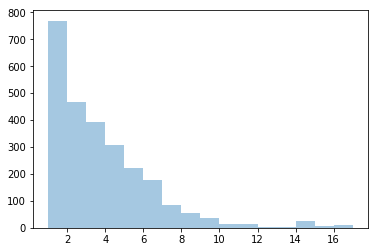
\includegraphics[width=0.45\textwidth]{img/before_slash_distribution}
        \label{fig:before_slash_distribution}
    }
    \caption{The distribution of the number of values per patent for assignee and \gls{ipc} class.}
    \label{fig:list_distribution}
\end{figure}

Using glyphs results in continuous areas with the same glyph appearance (see \autoref{fig:glyphs_areas}), which allows the users to make generalized assumptions about the content of those areas.
We evaluate how well glyphs fulfill their purpose in \autoref{subsubsec:hypothesis2}.
For simplicity, we refer to glyphs as points whenever the multiple attribute values are not essential to the current discussion.

\begin{figure}[!]
\centering
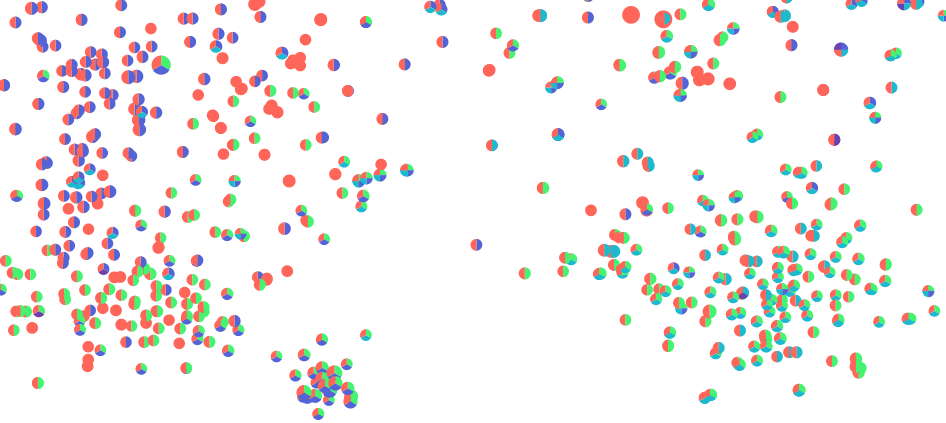
\includegraphics[width=\textwidth]{img/glyphs_areas}
\caption{Areas consisting of same kinds of glyphs on the contact lens dataset.}
\label{fig:glyphs_areas}
\end{figure}

\paragraph{Connections}~\\
Three kinds of possible connections between any pair of patents exist (see \autoref{fig:lines}).

\begin{figure}[!]
\centering
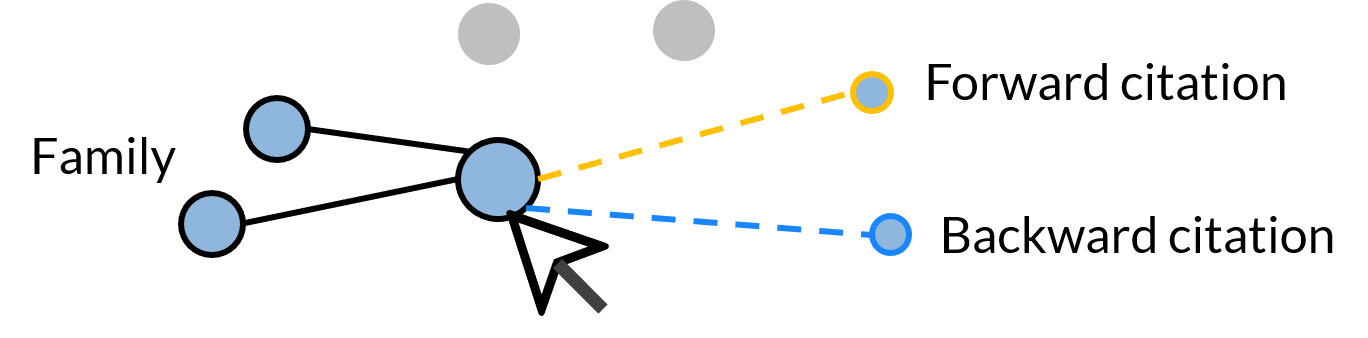
\includegraphics[width=0.7\textwidth]{img/lines}
\caption{Various kinds of connections between patents.}
\label{fig:lines}
\end{figure}

As described in \autoref{subsubsec:patent_family_and_priority_document}, patent families describe the same invention.
Being the same family is the strongest indication of a semantic similarity, which is why families mostly are represented by close-knit groups of points in our semantic approach.
We show connections to other family members with black solid lines.

Citations are another kind of possible connection between patents.
As opposed to family connections, they do have a direction.
Conventionally directed connections are shown with arrows, which is inapplicable in our case.
A single patent might have tens to hundreds of citations, which would result in a very cluttered representation if arrows were used.
Moreover, it is useful to be able to see at a glance the areas where the majority of citations come from and go to.
As described \autoref{subsubsec:forward_backward_citations}, if a new patent application cites an existing patent, it means the inventors are aware of the prior invention and see the novelty in their invention with regards to the prior invention.
This is called \textit{forward citation}, which we show with a yellow dashed line.
The opposite situation, i. e. from the point of view of an older patent, is a \textit{backward citation} shown with a blue dashed line.

We chose complementary colors (blue and yellow) because they signify exactly opposite things - opposite directions of citation.
Yellow is more of an ``active'' color, which signifies that currently selected patent explicitly mentions the citation.
Blue has a more ``passive'' role, which in our case corresponds to the fact that backward citations are not directly contained in the data, but are instead computed by reversing the connections.
Notably, yellow and blue both can be easily seen on black background.
It so happens that some patents are listed as both family members and citations, so dashed lines are designed to overlay the black lines and still be clearly distinguishable.
Additionally, a dashed line is usually perceived as less important than a solid line, which correctly represents the domain knowledge in this case.

Connections appear while the user is hovering over a patent with a mouse.
The user can also choose to select a patent by clicking on it.
In this case, the connections persist until the user switches their selection to another patent or resets the selection completely by clicking on the background area of the scatter plot.
The selection mode allows the user to highlight a patent of choice and examine its citations and family by hovering the mouse over them.
This interaction implements the principles of \textit{focus plus context} (explained in \autoref{subsubsec:focus_context}) and \textit{details on demand} (explained in \autoref{subsubsec:visual_information_seeking_mantra}).
The chosen patent is in focus and its citations and family provide a more detailed representation and also show some context, i. e. what prior art the patent refers to.

\paragraph{Labels}~\\
Each patent has a corresponding label that shows up to three top key terms as extracted by the TF-IDF algorithm (see  \autoref{subsec:term_extraction} for details).
Information density is an essential characteristic of any user interface that directly impacts usability.
To avoid cluttering the visualization space, we use use a heuristic to determine exactly what labels are shown and how many top key terms they include.

Our experiments showed that about 250 labels (consisting of one key term) for points can be shown simultaneously and remain mostly readable. 
So we decided to limit the labels to a maximum of 250.
This means that some points are shown unlabeled until the user restricted the area they are interested in to under 250 patents.
After each operation, such as filtering, panning or zooming, we count the points that are currently situated within the viewport.
We then divide that amount by 250.
If the resulting quotient $q$ is over 1, we round it up to the next integer to get $n$.
In this case, every $n$th point is labeled with its top key term. 
For example, if 980 patents are currently visible, every 4th of them gets labeled, and three-fourths of patents are shown with just a point without a label.
If $q$ is between 0.7 and 1, every patent in view is labeled with its top key term.
Usually, this happens during the examination of small clusters (see \autoref{subsec:hierarchical_clustering} for explanation of three cluster sizes), when the user's attention shifts to a single document.
For values of $q$ between 0.3 and 0.7, there is sufficient space for top two key terms and for values under 0.3 for three top key terms for every patent.

The above-mentioned value intervals are chosen to maintain a visual balance between points and their labels and to minimize overlapping text.
If the user wishes to examine further key terms beside the top three ones, they have the possibility to inspect them in the detail view (described in \autoref{subsec:detail_view}) along with complete information about the patent.
We provide the possibility for the user to comprehend the distribution of points and their colors without distraction before starting with the detailed analysis. 
To support this, we make all point labels invisible when the zoom level is less than 1.15.

The varying number and length of patent key terms result in a dynamic level of detail.
It is one of our multiple embodiments of the \textit{semantic zooming} mechanism (explained in \autoref{subsubsec:semantic_zooming}).
The evaluation (see \autoref{subsubsec:hypothesis5}) showed that our heuristic resulted in a readable representation for multiple levels of detail.

\paragraph{Zooming}~\\
Zooming causes a multiplicator to be applied to the point size.
The multiplicator value varies from 1x to 1.7x and is interpolated linearly depending on the exact zoom level.
The maximal possible zoom level is 10, but after it reaches 3, points and text in the scatter plot stop increasing in size, so further magnification only increases the distance between the points.
Thus, we intentionally increase the amount of white space to allow the user to focus their attention on specific patents.
Also, at this detail level, the documents are accompanied by a list of key terms which need to be readable.
Improved readability is also a reason for the additional white space.

The lines representing families and citations also change subtly with the zoom level.
Their width changes from 2 to 3 pixels to stay in proportion with the point size.

To allow users to quickly go back to the overview of the dataset, we added a ``Reset zoom'' button in the latest iteration of the concept.
This way, the users are able to go set the zoom level back to 1 with one click instead of turning the mouse wheel two to seven times depending on the size of the dataset.
We would like to mention that navigating to the maximum zoom level is rarely, if ever, continuous.
The user pauses to analyze the currently presented information to steer their further examination.
Therefore zooming into the dataset is not as cumbersome as zooming out without using the reset button would be.

\subsubsection{Clusters}
\label{subsubsec:clusters}
As described in \autoref{subsec:hierarchical_clustering}, we cluster patents hierarchically based on their distance in the 2D space, i. e. their proximity in the scatter plot.
From the computed agglomerative clustering we pick three specific cluster configurations, which provides us with three levels of detail.
We refer to them as \textit{large, medium} and \textit{small} cluster sizes.

Clusters are represented in the visualization by their key terms.
Since we are essentially generating a themescape, we considered a solution from the domain of map drawing.
On a map, labels for areas such as forests, deserts or lakes are often not straight but bent to match the shape of the area.
We tried to replicate this behavior by approximating the points in the cluster by a polynomial curve.
The cluster text was supposed to stretch and follow the curve to make the shape of the cluster visible.
The result of our attempts is presented in \autoref{fig:curves}.

\begin{sidewaysfigure}[!]
\centering
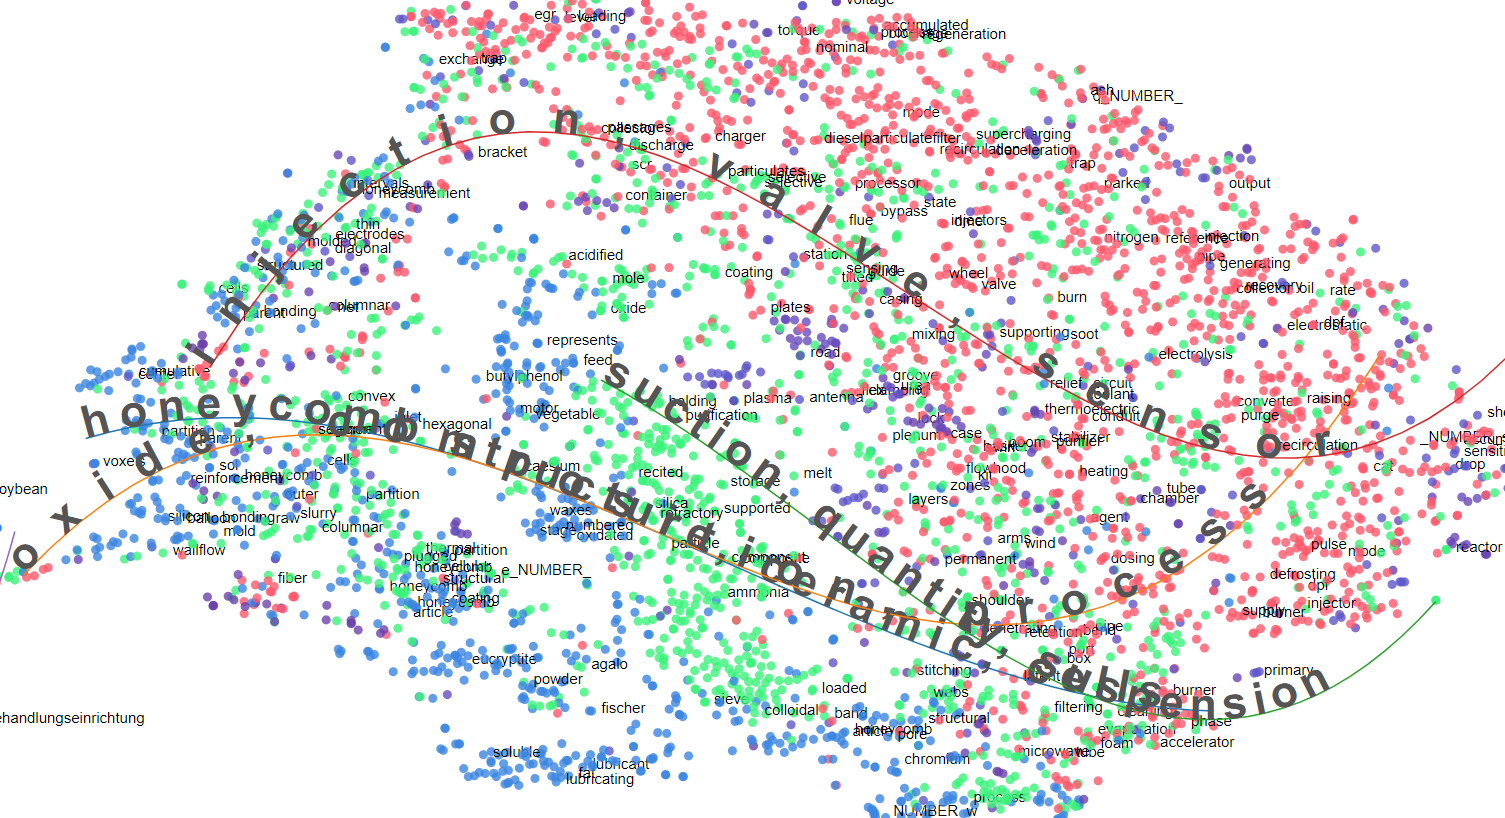
\includegraphics[width=\textwidth]{img/curves}
\caption{Cluster shapes approximated by curves on the diesel engine dataset. The text for cluster labels is placed on the curves.}
\label{fig:curves}
\end{sidewaysfigure}

At that stage, we were computing the whole clustering based on distances in the high-dimensional document space.
With this approach, dimension reduction to 2D resulted in elongated cluster shapes which, as we initially hoped, would be easy to approximate.
At the same time, elongated clusters were not separated clearly and often overlapped, which significantly reduced the quality of the approximating curves and the readability of text placed on them.
It was also difficult to adjust how the text should stretch depending on the length of the key terms and the length of the curve.
For these reasons, we decided not to pursue this direction of research further.
Notably, \cite{Skupin2013} uses the professional \gls{gis} software ArcGIS extended by the Maplex labelling engine to place labels on their themescapes with great success (see \autoref{fig:som} for an example themescape).
This speaks strongly for the potential of applying map drawing methods for non-geographical data.

In the current embodiment of our approach, each cluster is represented by its top three key terms situated exactly in the middle of the cluster.
To place them in a compact way, we show the most relevant term in the middle and complement it by the second and third terms above and below it.
The font size of the top term is bigger by three pixels to emphasize its importance according to principles of visual hierarchy.
Moreover, both visibility and font size differ between large, medium and small cluster labels depending on the current zoom level (see \autoref{table:font_sizes}).

\begin{table}[h!]
\centering
\begin{tabular}{||c c c||} 
 \hline
 Cluster level & Font size, pixels & Visible at zoom level \\ [0.5ex] 
 \hline\hline
 large & 23 to 28 & <1.6 \\ 
 medium & 18 to 22 & 1.5 to 2.1 \\
 small & 14 to 18 & 2.0 to 3 \\ [1ex] 
 \hline
\end{tabular}
\caption{Font sizes for different cluster sizes}
\label{table:font_sizes}
\end{table}

As the user zooms into the scatter plot, bigger clusters are replaced by smaller ones. 
This continues until the zoom level of 3, when the cluster labels disappear completely allowing the user to examine specific patents efficiently.
Notably, the visibility intervals overlap slightly.
This means that briefly, both large and medium or both medium and small cluster labels are seen.
The idea here is to make the transition between different levels of detail smoother.
The font size of cluster labels increases slightly while zooming in.
As mentioned before, points themselves and connections between points also increase in size.
This behavior is implemented in a consistent way throughout the scatter plot to support the feeling of ``moving into'' the dataset.

To optically balance out the increasing line thickness as the clusters labels become larger, we vary the font color slightly.
Labels for single patents are black, so we made little cluster labels a few shades lighter, which yields a dark gray.  
By analogy, medium and large clusters were also assigned gray color slightly lighter than at the corresponding previous level.
A comparison of black and our lighter alternative for large cluster labels can be seen on figures \autoref{fig:cluster_terms_black} and \autoref{fig:cluster_terms_gray}.
Additionally, the distinction between cluster terms and patent terms is accentuated by using unequal colors.
To strengthen the effect and increase readability on a colorful background, we draw a thin white contour around the cluster labels (compare figures \autoref{fig:cluster_terms_nowhite} and \autoref{fig:cluster_terms_gray}).

\begin{figure}
    \centering
    \subfigure[Black text with white contour]
    {
        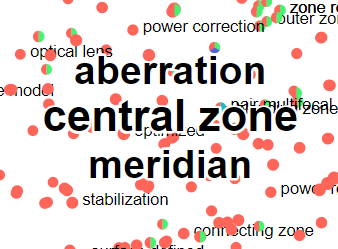
\includegraphics[width=0.4\textwidth]{img/cluster_terms_black}
        \label{fig:cluster_terms_black}
    }
    \subfigure[Gray text without contour]
    {
        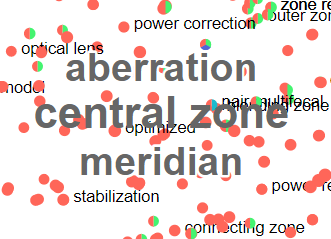
\includegraphics[width=0.4\textwidth]{img/cluster_terms_nowhite}
        \label{fig:cluster_terms_nowhite}
    }
    \subfigure[Gray text with white contour]
    {
        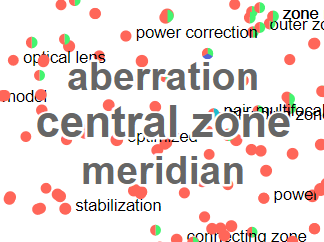
\includegraphics[width=0.4\textwidth]{img/cluster_terms_gray}
        \label{fig:cluster_terms_gray}
    }
    \caption{Font color and contour increase readability of cluster labels.}
    \label{fig:cluster_labels}
\end{figure}

Some of the cluster key terms are assigned a list of \textit{augmenting words} which provide context for occasionally unclear or ambiguous terms (see \autoref{subsec:hierarchical_clustering} for details on augmentation).
This information is not of a high-priority, thus we only display it on demand.
A tooltip with a list of augmenting words appears when and only when the user hovers over the corresponding term with the mouse.
No tooltip is shown when the given term possesses no augmenting words.
Naturally, there has to be a clear indication of what term out of three possible presented is enhanced with a tooltip.
There was no easy technical possibility to show the tooltip on the side of the corresponding term, so we placed it underneath the cluster label.
We make the current state of the interface explicit by highlighting in wine red color the term which the tooltip currently corresponds to as shown in \autoref{fig:tooltips}.

\begin{figure}[!]
\centering
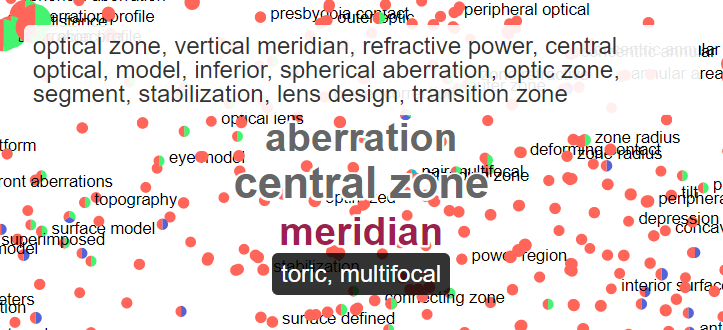
\includegraphics[width=0.8\textwidth]{img/tooltips}
\caption{Tooltip with augmenting words below and tooltip with all cluster terms above}
\label{fig:tooltips}
\end{figure}

Since we actually computed the top 15 key terms per cluster but had only been showing 3 of them so far, we decided to display the remaining 12, too.  
For that purpose, in the latest iteration of the prototype we added another tooltip, this time above the three terms, with distinctly different appearance to avoid any confusion.
The interaction follows the same pattern as with the first tooltip, i. e. it is displayed on mouse hover.

\subsection{Histogram}
\label{subsec:histogram}

The histogram view shows the number of submitted patent applications per year in the form of a bar chart (see \autoref{fig:histogram}).
It is, in fact, a histogram in which the bin size equals one year.
It allows the user to involve the temporal dimension into their perception of the data.
With a brushing interaction, the user can filter out the data outside the selected interval.
The selected window can be moved or expanded with the help of the handles on either side.
With a click on the background of the histogram the selection can be reset.
On the X-axis, only every second year is labeled to avoid overcrowding.
To compensate for that, the years of a current selection are shown in the upper-left corner.
It helps eliminate the need for mental computations as the user chooses a time interval of interest.

\begin{figure}[!]
\centering
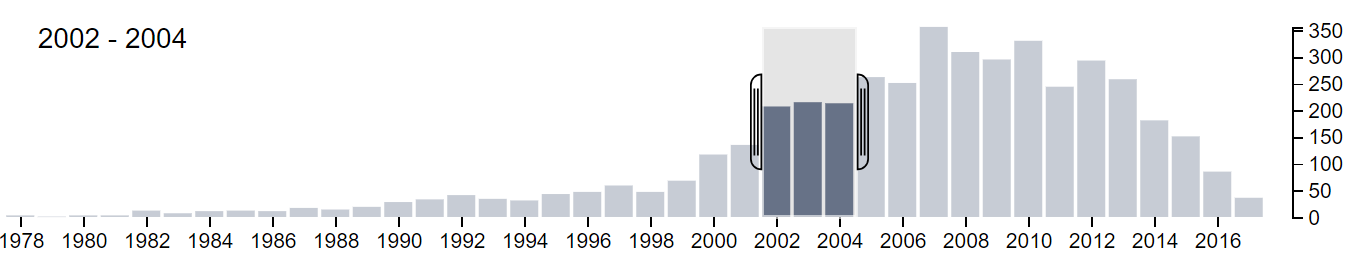
\includegraphics[width=\textwidth]{img/histogram}
\caption{Histogram view as seen on diesel engine dataset. The time interval from 2002 to 2004 is selected.}
\label{fig:histogram}
\end{figure}

The values in the histogram are computed based on the current top node in the sunburst.
Initially, the top node corresponds to the whole dataset, and then switches to its specific portions as the user focuses their attention on specific metadata attribute values.
The scale of the Y-axis of the histogram is adjusted dynamically as its maximum value changes.
Additionally, the histogram is directly involved in other forms of interactions between views that are described in \autoref{sec:interactions_between_views}.

\subsection{Sunburst and breadcrumbs}
\label{subsec:sunburst_and_breadcrumbs}

\subsubsection{Sunburst}
\label{subsubsec:sunburst}
Our implementation of sunburst is based on interactive demos from \cite{Asturiano} and \cite{Trott}.
The angle taken by nodes is linearly dependent on the number of patents that have the corresponding attribute value.
The nodes are sorted by their value in the descending order.
When there is enough space available, node names are displayed in the center of a node.
The text follows the node's arc and is surrounded by a white contour for a better readability.
The title of the node and an absolute number of patents belonging to it are also shown as a tooltip when the user hovers over the node.

The color of nodes on the first sunburst level is based on a cyclical rainbow color palette.
Basically, the angles within the interval $[0\textdegree, 360\textdegree]$ are mapped to a corresponding position from $[0, 1]$ on the color scale.
A node's angle for the purpose of this calculation starts at 0\textdegree and ends in the middle of the node's arch where its title is.
Because the color scale is cyclical, nodes nearing 360\textdegree have similar colors to those near 0\textdegree.
Child nodes expanding from the first sunburst level are assigned a spectrum of shades from darker than parent to lighter than parent.
This emphasizes that they belong to the parent.

When patents possess multiple values of the same attribute, for example, assignee or \gls{ipc} class, occurrences of each single value are bound to exceed the number of patents when summed up.
To represent that overlap correctly, we normalize the values so that they add up to a total of 100\%.
For example, assume there are two assignees A and B in a dataset, 80\% of patents have A as their assignee and 40\% have B.
This means that 20\% of patents have been submitted by A and B together.
To correctly represent the relative distribution, we would draw node A as $\frac{80}{80+40=120} = 67\%$ of the sunburst and node B as $\frac{40}{120} = 33\%$.

It is possible to navigate to deeper hierarchy levels by clicking on the chosen node.
To go back one level, the user needs to click on the circle in the middle of the sunburst which represents the current top node.
The transitions between two states are animated to emphasize the change in the system state: sunburst nodes fold and unfold like a fan.
Change in the state of the sunburst also directly affects the scatter plot: first, only points belonging to the currently chosen node stay visible, second, their colors change to match the new sunburst nodes.
In addition to clicking, the user can also hover over a sunburst node to see a preview of their choice.
In this case, not related patents are hidden in the same way as with clicking, but point colors stay as they are because the sunburst nodes have not yet changed their colors.
Only the nodes on the path to the currently highlighted node retain their color.
Remaining nodes are shown with a lighter color to keep all focus on the highlight.
The highlight is reset after the user moves the mouse outside of the sunburst's circle.

\subsubsection{Breadcrumbs}
\label{subsubsec:breadcrumbs}
\textit{Visibility of system status} and \textit{recognition over recall} are two of usability expert Jakob Nielsen's ten heuristics for user interface design \cite{Nielsen1994}. 
To take them into account, the first change from the initial concept was adding \textit{breadcrumbs} to the sunburst view.

Breadcrumbs are a metaphor most familiar to users from website navigation (see \autoref{fig:breadcrumb_examples} for examples).
The name originates from the German fairy tale about Hansel and Gretel, who left a trail of bread crumbs in the woods to be able to find their way back \cite{levene2011introduction}.
Breadcrumbs are applicable with hierarchically arranged navigation, i. e. when there is only one possible path to every node in the navigation tree.
According to \cite{Gube2019}, they are usually used as an optional aid to navigation and should be less prominent than the primary navigation element (which is the sunburst in our case).

\begin{figure}[!]
\centering
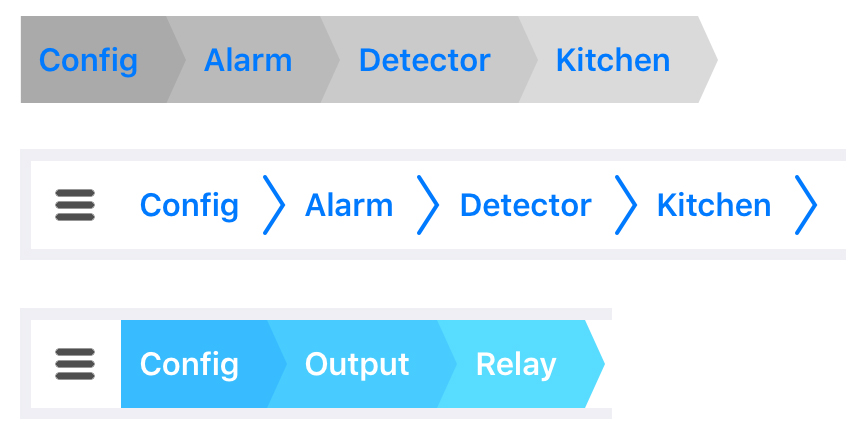
\includegraphics[width=0.5\textwidth]{img/breadcrumb_examples}
\caption{Different kinds of breadcrumb design. Image source:\cite{breadcrumb}}
\label{fig:breadcrumb_examples}
\end{figure}

With the first implementation of the sunburst, it soon became clear that some hierarchy nodes were too narrow to include their title within.
Moreover, the titles that could be shown were placed at different angles, which prevented a sequence of highlighted nodes from being read easily.
Breadcrumbs build a straight line, which increases readability.
Additionally, when a user switches to a deeper level of the sunburst hierarchy, the parent nodes are no longer visible. 
In accordance with the \textit{recognition over recall} principle, it should not be expected of any user to remember what parent nodes came before.
We included breadcrumbs as a visual aid that clearly and consistently represents the status of the system and reassures the users of the result of their actions, especially when they interact with small sunburst nodes.
The result can be seen in \autoref{fig:breadcrumbs_without_text}.
A percentage on the right side of the breadcrumb trail represents the fraction of patents from the currently highlighted hierarchy node with regard to the current root node.
It is especially useful when there is a significant overlap between node values because it shows the true value of the node independent of its normalized angle.

\begin{figure}[!]
\centering
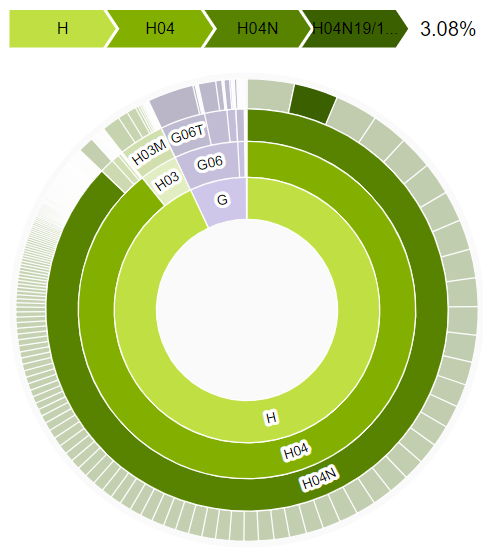
\includegraphics[width=0.7\textwidth]{img/breadcrumbs_without_text}
\caption{First version of breadcrumbs complementing the sunburst view.}
\label{fig:breadcrumbs_without_text}
\end{figure}

Short codes for \gls{ipc} classes fit well into the width of the line allocated to them.
To keep the breadcrumbs view concise for assignees as well, we chose only to show the first nine characters of a node's title followed by an ellipsis mark.
As assignee names can be over 30 characters long, the need to see full node titles remains.
The idea proposed by patent experts during a feedback meeting helped address this issue.
The experts wished to see full descriptions for \gls{ipc} codes, for example, ``optical elements, systems, or apparatus'' for class G02B (see \cite{ipc} for full schema).
This led us to complement the graphical brief breadcrumbs with a full-text part as seen in \autoref{fig:breadcrumbs_text}.
Full assignee names could then be shown completely along the \gls{ipc} descriptions.

\begin{figure}[!]
\centering
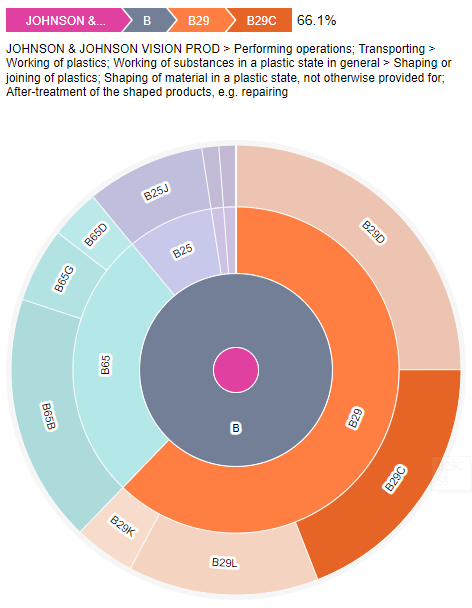
\includegraphics[width=0.8\textwidth]{img/breadcrumbs_text}
\caption{Full-text titles of sunburst nodes added to breadcrumbs.}
\label{fig:breadcrumbs_text}
\end{figure}

\subsection{Detail view}
\label{subsec:detail_view}

The detail view follows the principle of \textit{details on demand} (see \autoref{subsubsec:visual_information_seeking_mantra} for details). 
It allows the user to examine all of the available metadata per patent.
The information is organized in a tabular manner for compactness (see \autoref{fig:detail_view}).
Included are (left to right, top to bottom) publication number, title, application date, a list of assignees, forward and backward citations, a list of \gls{ipc} classes,  a list of the top 15 relevant key terms and the abstract.

\begin{figure}[!]
\centering
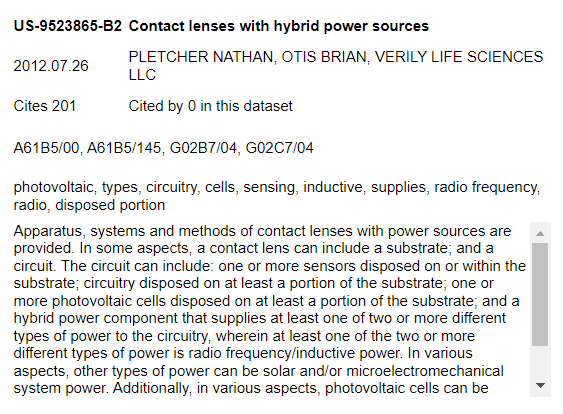
\includegraphics[width=0.8\textwidth]{img/detail_view}
\caption{Detail view on an example patent from the contact lens dataset.}
\label{fig:detail_view}
\end{figure}

If the user would like to study the patent text thoroughly, they can double-click anywhere in the detail view.
This causes an additional browser window to appear, which contains the full text of the textual parts of the patent, i. e. abstract and claims (see \autoref{fig:claims}).
When the user double-clicks on another patent, the already opened window persists and a new one is opened.
This permits a detailed examination and comparison of multiple patents.

\begin{figure}[!]
\centering
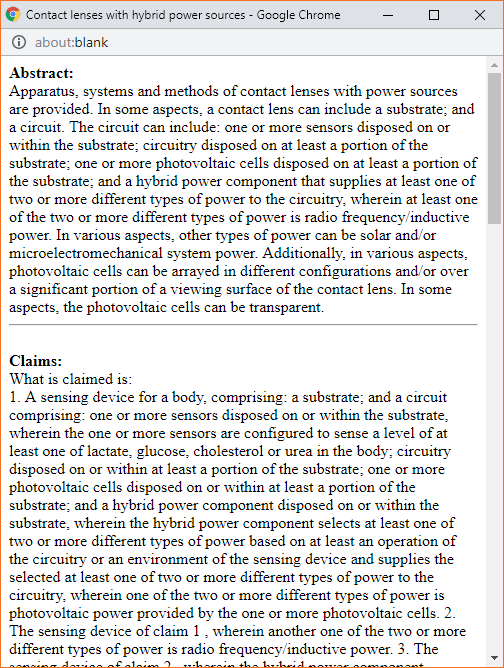
\includegraphics[width=0.8\textwidth]{img/claims}
\caption{Window with full text (abstract and claims) of an example patent from the contact lens dataset.}
\label{fig:claims}
\end{figure}

\subsection{Interactions between views}
\label{sec:interactions_between_views}

For a consistent behavior across all parts of the interface, we enable similar kinds of interactions for the sunburst, the histogram and the scatter plot.
We distinguish between three kinds of interactions:
\begin{itemize}
\item hovering over an object for a preview of the changes - ``Highlighting''
\item clicking on an object to make the change persistent - ``Selecting''
\item clicking on a background of the view to reset the selection.
\end{itemize}
An overview of how those interactions influence coordinated views is shown in \autoref{fig:interactions_between_views}.
In this section we describe the possible user actions that had not yet been covered in the previous sectionss.

\begin{figure}[!]
\centering
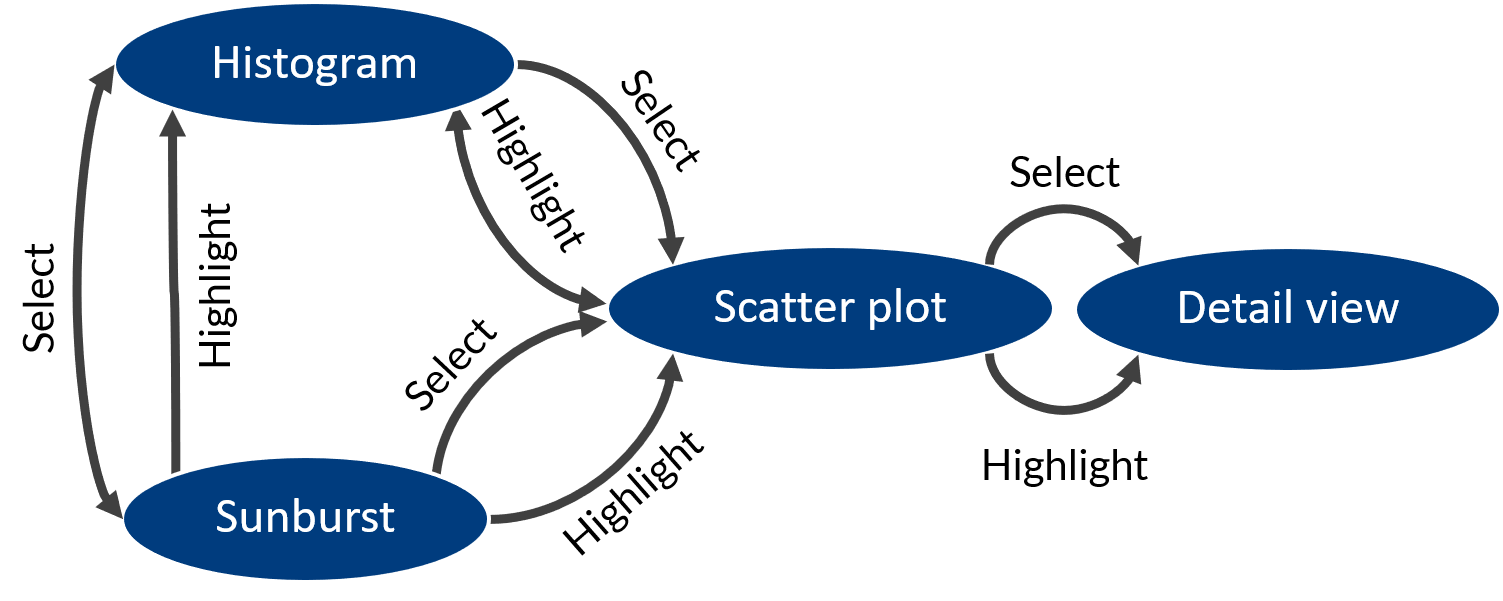
\includegraphics[width=0.8\textwidth]{img/interactions_between_views}
\caption{Diagram of interactions between views. The arrows point from the view where the given interaction happens to the view where it takes effect.}
\label{fig:interactions_between_views}
\end{figure}

On a histogram, the user can select a certain time interval by brushing.
The histogram bars for the years outside the selection become grayed out, so do the patents submitted outside the selected interval.
Then, the sunburst is generated anew based only on the patents within the selection.
The colors of the remaining points then adjust to match the new state of the sunburst.
See \autoref{fig:histogram_brushing_interaction} for a comparison of states before and after brushing.
In this example, one can see that patents submitted from 2007 to 2011 are concentrated in one thematic area.
Moreover, less of them are assigned the \gls{ipc} class G - ``Physics'', while H - ``Electricity'' becomes more widespread.
This might be an indication of a change in the meaning of the \gls{ipc} classes over time: the first version of \gls{ipc} classification was developed in 1968 before the rapid development of information technology.
The selection in the histogram can be reset by clicking on its background.

\begin{figure}[!]
    \centering
    \subfigure[Before brushing]
    {
        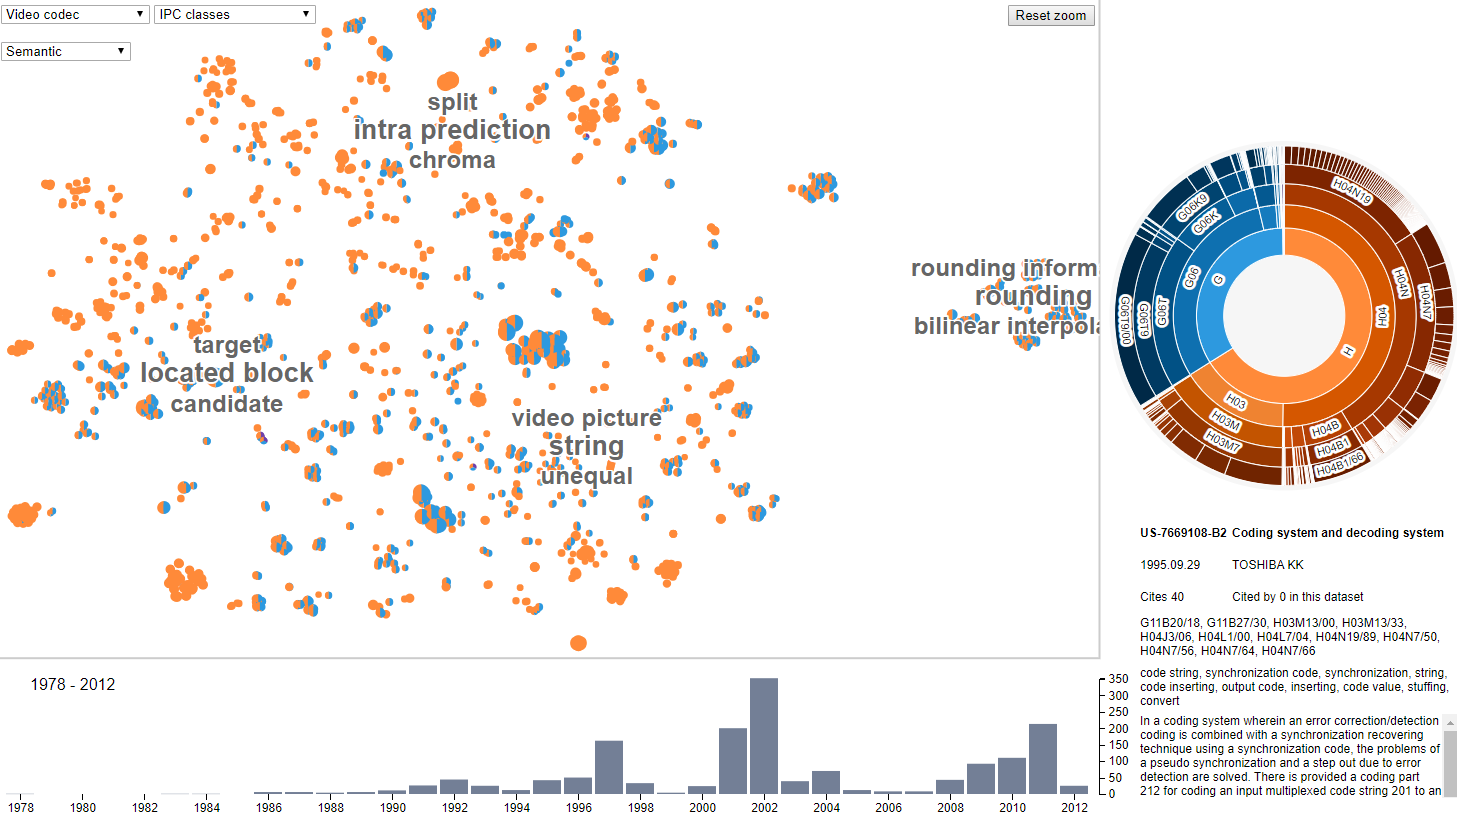
\includegraphics[width=\textwidth]{img/histogram_before_brush}
        \label{fig:histogram_before_brush}
    }\\
    \subfigure[After brushing]
    {
        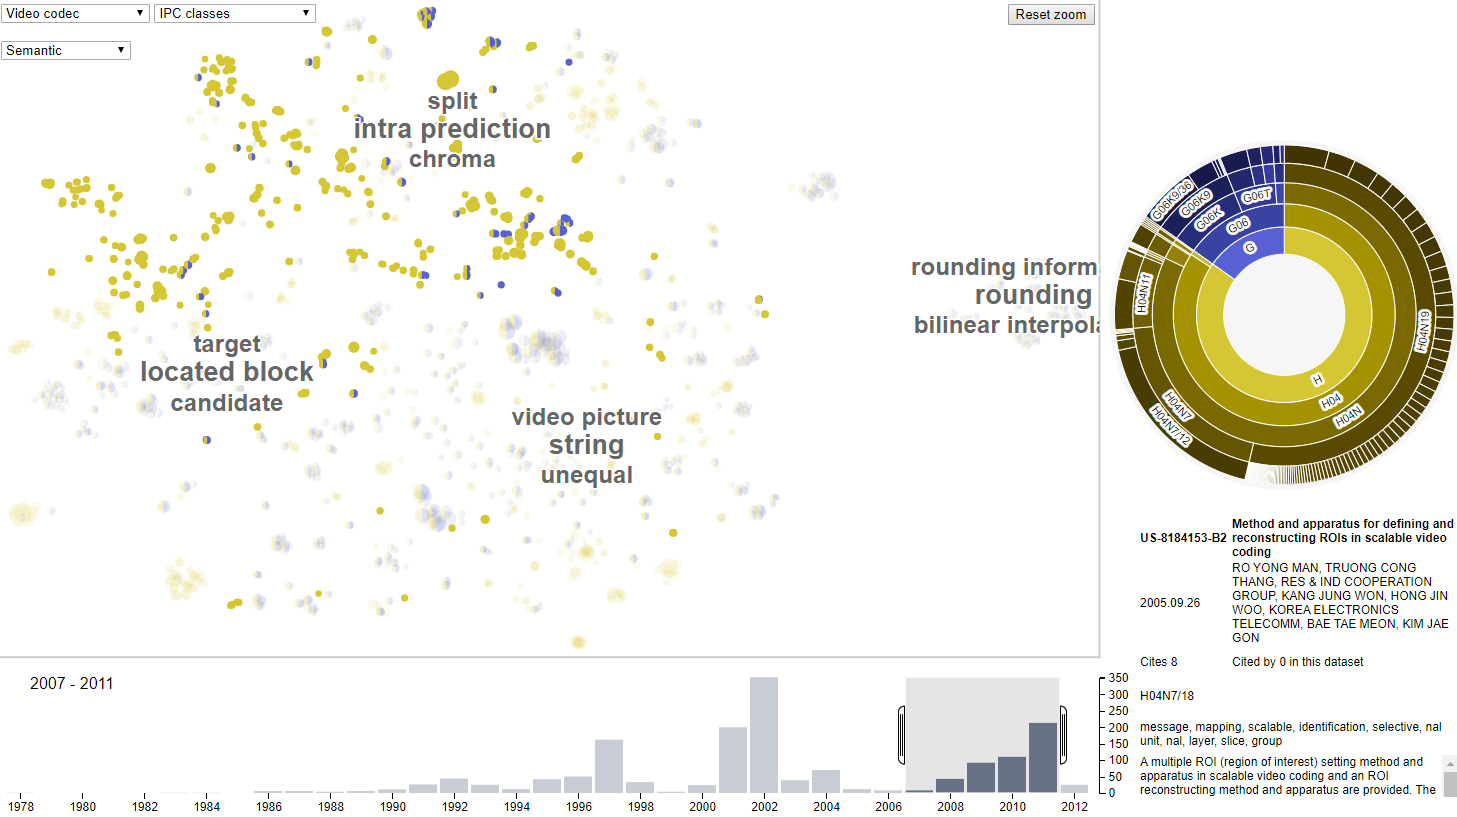
\includegraphics[width=\textwidth]{img/histogram_after_brush}
        \label{fig:histogram_after_brush}
    }
    \caption{The impact of a brushing action on a histogram on the scatter plot and sunburst. Video codec dataset}
    \label{fig:histogram_brushing_interaction}
\end{figure}

When the user hovers over a sunburst node, this node's contribution to the histogram is displayed in the color corresponding to the sunburst node.
In other words, the histogram becomes a stacked bar chart in which the bottom part of the stack corresponds to the highlighted sunburst node and the upper part of the stack includes all other patents.
This interaction allows the user to follow the temporal trends in the development of a single \gls{ipc} class, assignee or country.
For example, Figure \autoref{fig:sunburst_hover} shows that 3D printing technology has started developing rapidly in China since 2015.
If the user then clicks on China, it moves to the center of the sunburst and its children take over the whole circle.
The bars corresponding to China that were blue on hover now constitute the whole histogram and the Y-axis is scaled accordingly (see Figure \autoref{fig:sunburst_click}).
Moreover, the points in the scatter plot now match their colors to the child nodes of China.

\begin{figure}[!]
    \centering
    \subfigure[While hovering]
    {
        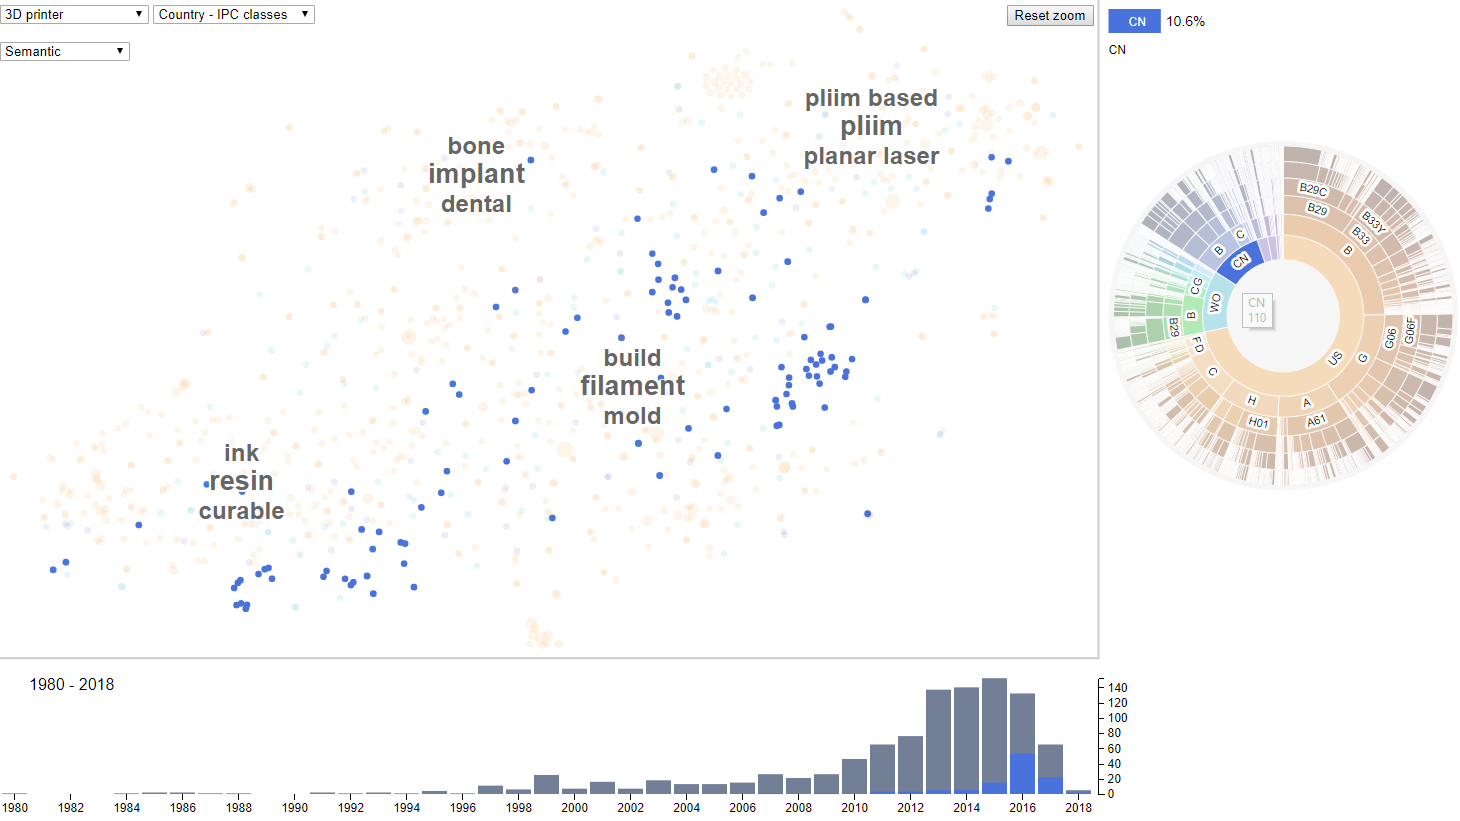
\includegraphics[width=\textwidth]{img/sunburst_hover}
        \label{fig:sunburst_hover}
    }\\
    \subfigure[After clicking]
    {
        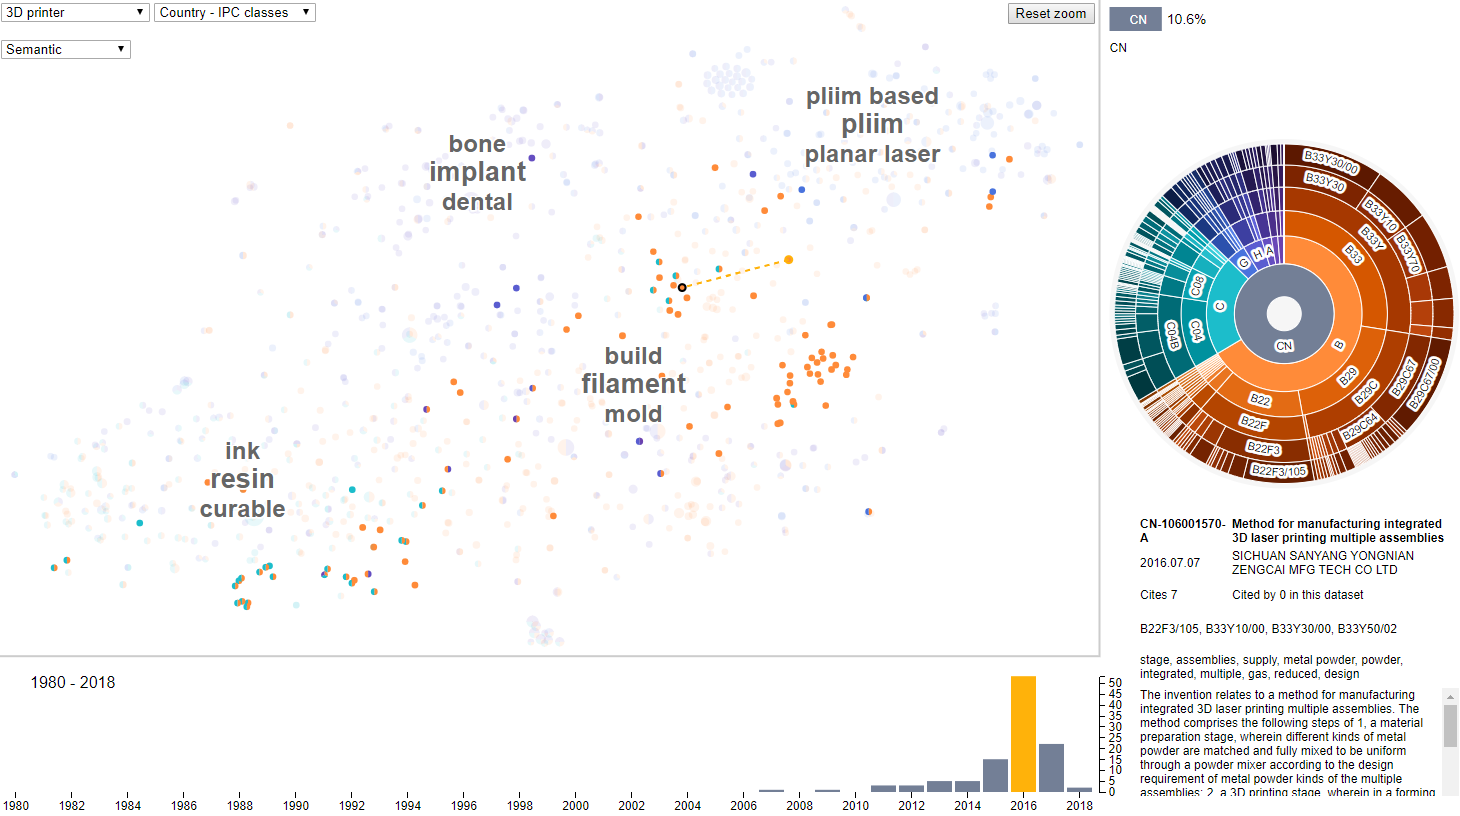
\includegraphics[width=\textwidth]{img/sunburst_click}
        \label{fig:sunburst_click}
    }
    \caption{The impact of hovering and clicking on a sunburst node on histogram and scatter plot. 3D printer dataset}
    \label{fig:sunburst_interactions}
\end{figure}

The scatter plot also implements the highlighting and selection with regard to single patents.
As long as the user hovers over a certain point, it is emphasized by a black contour and its citations and family members become visible.
The detail view then shows the metadata of this particular point, but the information persists even when the mouse is taken away until some other patent is highlighted.
Moreover, the year when the patent was submitted is accented in bright yellow on the histogram (see Figure \autoref{fig:sunburst_click}).
It gives the user a quick impression about the age of the patent without the need to read this information in textual form in the detail view.
Clicking on a patent makes its connections permanently visible.
The user is then able to examine related patents by hovering over them.
The detail view is reset to the details of the selected point when no other point is hovered over.
A click on a background of the scatter plot resets its selected point.

All above-mentioned interactions between linked views taken together allow the user to focus their attention on any desired aspects of the data, be it the temporal aspect or specific metadata values.
The display can be restricted to a region of interest by various filters.
We made an effort to enable interactions on both micro- and macrolevel (for single patents and for groups of various sizes).
Users' understanding of the interplay between views is evaluated in \autoref{subsubsec:hypothesis4}.